\documentclass[12pt]{article}
\usepackage{amsmath}
\usepackage{amssymb}
\usepackage[letterpaper,margin=0.85in,centering]{geometry}
\usepackage{fancyhdr}
\usepackage{enumerate}
\usepackage{lastpage}
\usepackage{multicol}
\usepackage{graphicx}
\usepackage{vwcol}
\reversemarginpar

\pagestyle{fancy}
\cfoot{Page \thepage \ of \pageref{LastPage}}\rfoot{{\bf Total Points: 100}}
\chead{MATH 1560}\lhead{FINAL EXAM}\rhead{20th June, 2017}

\newcommand{\points}[1]{\marginpar{\hspace{24pt}[#1]}}
\newcommand{\skipline}{\vspace{12pt}}
%\renewcommand{\headrulewidth}{0in}
\headheight 30pt

\newcommand{\di}{\displaystyle}
\newcommand{\abs}[1]{\lvert #1\rvert}
\newcommand{\R}{\mathbb{R}}
\newcommand{\C}{\mathbb{C}}
\renewcommand{\P}{\mathcal{P}}
\DeclareMathOperator{\nul}{null}
\DeclareMathOperator{\range}{range}
\DeclareMathOperator{\spn}{span}
\newcommand{\len}[1]{\lVert #1\rVert}
\newcommand{\Q}{\mathbb{Q}}
\newcommand{\N}{\mathbb{N}}
\renewcommand{\L}{\mathcal{L}}
\newcommand{\dotp}{\boldsymbol{\cdot}}
\newenvironment{amatrix}[1]{%
  \left[\begin{array}{@{}*{#1}{c}|c@{}}
}{%
  \end{array}\right]
}
\newcommand{\bam}{\begin{amatrix}}
\newcommand{\eam}{\end{amatrix}}
\newcommand{\bbm}{\begin{bmatrix}}
\newcommand{\ebm}{\end{bmatrix}}

\begin{document}


\author{Instructor: Sean Fitzpatrick}
\thispagestyle{plain}
\begin{center}
\emph{University of Lethbridge}\\
Department of Mathematics and Computer Science\\
20th June, 2017, 9:00 am - 12:00 pm\\
{\bf MATH 1560 - FINAL EXAM}\\
Examiner: Sean Fitzpatrick
\end{center}
\skipline \skipline \skipline \noindent \skipline
Last Name:\underline{\hspace{350pt}}\\
\skipline
First Name:\underline{\hspace{348pt}}\\
\skipline
Student Number:\underline{\hspace{322pt}}\\
\skipline



\vspace{0.1in}


\begin{quote}

 
 Record your answers below each question in the space provided.    Left-hand pages may be used as scrap paper for rough work.  If you want any work on the left-hand pages to be graded, please indicate so on the right-hand page. Additional scrap paper may be requested if needed.
 
 \bigskip
 
 Partial credit will be awarded for partially correct work, so be sure to show your work, and include all necessary justifications needed to support your arguments. 

\bigskip

 A basic (non-graphing, non-programmable) calculator is permitted. All other outside aids, including, but not limited to, mobile phones, textbooks, computers, drones, elves, and scrap paper, are prohibited.
\end{quote}


\bigskip

For grader's use only:

\begin{table}[hbt]
\begin{center}
\begin{tabular}{|l|r|} \hline
Page&Grade\\
\hline \hline
\cline{1-2} 2 & \enspace\enspace\enspace\enspace\enspace\enspace/10\\
\cline{1-2} 3 & \enspace\enspace\enspace\enspace\enspace\enspace/10\\
\cline{1-2} 4 & \enspace\enspace\enspace\enspace\enspace\enspace/10\\
\cline{1-2} 5 & \enspace\enspace\enspace\enspace\enspace\enspace/10\\
\cline{1-2} 6 & \enspace\enspace\enspace\enspace\enspace\enspace/10\\
\cline{1-2} 7 & \enspace\enspace\enspace\enspace\enspace\enspace/10\\
\cline{1-2} 8 & \enspace\enspace\enspace\enspace\enspace\enspace/10\\
\cline{1-2} 9 & \enspace\enspace\enspace\enspace\enspace\enspace/10\\
\cline{1-2} 10 & \enspace\enspace\enspace\enspace\enspace\enspace/10\\
\cline{1-2} 11 & \enspace\enspace\enspace\enspace\enspace\enspace/10\\
\cline{1-2} Total & \enspace\enspace\enspace\enspace\enspace\enspace/100\\
\hline
\end{tabular}

\end{center}
\end{table}
\newpage


\begin{enumerate}
\item For each limit below, evaluate the limit, or explain why it does not exist. (If a limit is infinite, indicate whether the value is $+\infty$ or $-\infty$.)
\begin{enumerate}
 \item $\di \lim_{x\to 2}\frac{x+3}{x^2+1}$. \points{2}

\vspace{1in}

 \item $\di \lim_{x\to 2}\frac{x-2}{x^2-4}$. \points{2}

\vspace{1in}

 \item $\di \lim_{x \to 0}\frac{\sin(5x)}{x}$. \points{2}

\vspace{1.5in}

 \item $\di \lim_{x \to 0}\frac{x\sin(x)}{1-\cos(x)}$ \points{2}

\vspace{1.5in}

 \item $\di \lim_{x\to 1}\frac{x^2-5x+6}{x^2-1}$ \points{2}

\end{enumerate}
\newpage

\item Let $f(x) = \dfrac{1}{x^2}$. \textbf{Using the definition of the derivative}, compute $f'(1)$. \points{4}


\vspace{3.5in}


\item The graph of a function $f$ is shown below. Give the values of the indicated limits:\points{6}

\bigskip


\begin{vwcol}[widths={0.6,0.4},
 sep=.8cm, justify=flush,rule=0pt,indent=1em]
\noindent\hglue-12pt 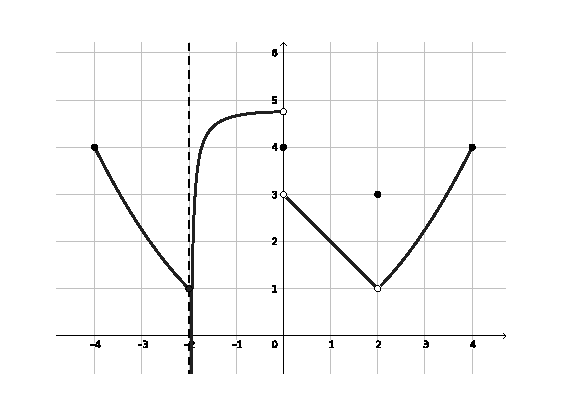
\includegraphics[width=0.6\textwidth]{FE-3}


$\di\lim_{x\to -2^-}f(x) = \underline{\hspace{1in}}$

\bigskip

$\di\lim_{x\to -2^+}f(x) = \underline{\hspace{1in}}$

\bigskip

$\di\lim_{x\to 0^-}f(x) = \underline{\hspace{1in}}$

\bigskip

$\di\lim_{x\to 0^+}f(x) = \underline{\hspace{1in}}$


\bigskip

$\di\lim_{x\to 2^-}f(x) = \underline{\hspace{1in}}$


\bigskip

$\di\lim_{x\to 2^+}f(x) = \underline{\hspace{1in}}$

\end{vwcol}

\medskip

For $a=-2$, $a=0$, and $a=2$, use your results above to determine whether or not $f$ is continuous at $x=a$. If not, indicate the type of discontinuity.

\medskip

At $a=-2$: 

\bigskip

\medskip

At $a=0$:

\bigskip

\medskip

At $a=2$:

\newpage

\item Compute the derivatives of the following functions:
\begin{enumerate}
 \item $\di f(x) = 3x^4-5x^2+\cos(x)+2\pi^3.$ \points{2}

\vspace{1.5in}

 \item $\di g(x) = e^x\tan(x)$ \points{3}

\vspace{1.75in}

 \item $\di h(x) = \frac{x^2+2x}{\sqrt{x}}$ \points{3}

\vspace{2.25in}

 \item $\di r(x) = \arcsin(x^3)$ \points{2}
\end{enumerate}
\newpage

\item Use implicit differentiation to find $\dfrac{dy}{dx}$ given that \points{4}
\[
 x^3y^2 = 4x-2y.
\]

\vspace{3in}

\item Compute the derivative of the following functions:
\begin{enumerate}
 \item $f(x) = \ln\left(\dfrac{x^3e^{x^2}}{\sqrt{x+1}}\right)$. \points{3}

\vspace{2in}

 \item $g(x) = x^x$ \points{3}
\end{enumerate}
\newpage

\item Let $f(x) = 6x^{1/2}-x^{3/2}$, for $x\in [1,4]$.\label{a}
\begin{enumerate}
 \item Find and classify all critical points of $f$. \points{4}
 \item Determine the absolute maximum and minimum of $f$ on the given interval. \points{1}
 \item Determine the intervals on which $f$ is increasing and decreasing.\points{1}
\end{enumerate}
\vspace{4in}

\item Repeat steps (a) - (c) in Question \ref{a} for the function $g$ whose graph is given below. \points{4}
\begin{multicols}{2}
 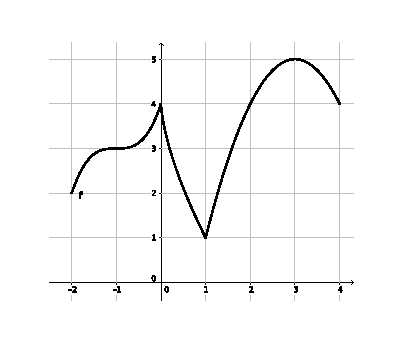
\includegraphics[width=0.95\columnwidth]{FE-8}
\end{multicols}

\newpage

\item Sketch the graph of the function $f(x) = \dfrac{x}{(x+3)^2}$. \points{10} \\
Your sketch doesn't have to be artistically perfect, but it should be large enough for me to see, and any intercepts, critical points, inflection points, and asymptotes must be clearly labelled.

In addition to your sketch, you should give the domain of $f$, as well as the intervals on which $f$ is increasing and decreasing, and concave up and concave down.

\newpage

\item The length of a rectangle is increasing at a rate of 8 cm/s, while its width is increasing at a rate of 3 cm/s. At what rate is the area of the rectangle increasing at the moment when its length is 20 cm and its width is 10 cm? \points{5}

\vspace{3.75in}

\item Find the dimensions of the rectangle of \textit{largest area} that can be drawn on the plane, if the base of the rectangle must lie on the $x$-axis, and the other two corners of the rectangle (above the $x$-axis) must lie on the parabola $y=8-x^2$.\points{5}

\newpage

\item Compute the degree three Taylor polynomial, centred at $a=0$, for the following functions:
\begin{enumerate}
 \item $f(x) = \sqrt{x+1}$ \points{4}

\vspace{3in}

 \item $\di g(x) = \int_0^x e^{-t^2}\,dt$ \points{4}
\end{enumerate}


\vspace{3in}

\item Determine a function $f(x)$ such that $f'(x) = 3x^2-\dfrac{3}{x^2}$ and $f(1)=3$.\points{2}
 
\newpage

\item Evaluate the following indefinite integrals:
\begin{enumerate}
 \item $\di \int (2x^3-\sqrt{x}+\cos(x))\,dx$ \points{2}

\vspace{1.5in}

 \item $\di \int\left(\frac{1}{x}+\frac{1}{x^2}+\frac{1}{x^2+1}\right)\,dx$ \points{2}

\vspace{1.5in}

 \item $\di \int \frac{e^{\sqrt{x}}}{\sqrt{x}}\,dx$ \points{3}

\vspace{2in}

 \item $\di \int \frac{\sin(x)}{\cos^2(x)}\,dx$ \points{3}
\end{enumerate}
\newpage

\item Evaluate the following definite integrals:
\begin{enumerate}
 \item $\di \int_1^e \frac{(\ln(x))^2}{x}\,dx$ \points{3}

\vspace{2.5in}

 \item $\di \int_2^6 x\sqrt{x-2}\,dx$ \points{3} (Hint: if $u=x-2$, then $x=u+2$...)
\end{enumerate}

\vspace{2.5in}

\item Express the integral $\di \int_0^4 x^2e^x\,dx$ as a limit of Riemann sums. You \textbf{do not} have to evaluate the limit.\points{4}

\end{enumerate}
\newpage

Extra space for rough work. And also, a unit circle.

\vspace*{\fill}

\begin{center}
 \includegraphics{UnitCircle}
\end{center}

\end{document}